\documentclass{article}
\input{../../../../format}
\lhead{Networks and Systems - Compiler Design}
\usepackage{minted}
\usepackage{hyperref}
\usepackage{enumerate}
\usepackage{boxedminipage}
\usepackage{xcolor}
\usepackage{tikz}
\usepackage{fancyvrb}
%\usepackage{hyperref}
\definecolor{links}{HTML}{2A1B81}
\hypersetup{colorlinks,linkcolor=,urlcolor=blue}
\usetikzlibrary{shapes.misc}
\usetikzlibrary{shapes.geometric, arrows, positioning}

\title{Systems Programming --- Lecture 14:\\
More on Pointers \& Coursework}
\author{Dr Konrad Dabrowski\\
\href{mailto://konrad.dabrowski@durham.ac.uk}{konrad.dabrowski@durham.ac.uk}
}
\date{E103 Christopherson Building}



\begin{document}

\begin{center}
	\underline{\huge Pointers and Coursework}
\end{center}



\section{Function Pointers}
\begin{itemize}
\item We've seen pointers to variables. We can also have pointers to functions!
\begin{minted}{c}
#include<stdio.h>
void hello_function(int times);

int main(){
  void (*func_ptr)(int);
  func_ptr=hello_function;
  func_ptr(3);
  return 0;
}

void hello_function(int times){
  for(int i=0;i<times;i++) {
    printf("Hello, World!\n");
  }
}
\end{minted}
\end{itemize}



\section{Using \texttt{qsort()}}
\begin{itemize}
\item \verb!stdlib.h! contains an implementation of the quicksort algorithm. The function declaration is:
\begin{minted}{c}
void qsort(void *base, size_t nmemb, size_t size,
    int (*compar)(const void *, const void *)) 
\end{minted}
\item \verb!void *base! is a pointer to the array
\item \verb!size_t nmemb! is the number of elements in the array
\item \verb!size_t size! is the size of each element
\item \verb!int (*compar)(const void *, const void *)! is a function pointer composed of two arguments and returns \verb!0! when the arguments have the same value, \verb!<0! when \verb!arg1! comes before \verb!arg2!, and \verb!>0! when \verb!arg1! comes after \verb!arg2!.
\end{itemize}



\begin{minted}{c}
#include <stdio.h>
#include <stdlib.h>
int compare (const void *, const void *); 
int main() {
  int arr[] = {52, 14, 50, 48, 13};
  int num, width, i;
  num = sizeof(arr)/sizeof(arr[0]);
  width = sizeof(arr[0]);
  qsort(arr, num, width, compare);
  for (i = 0; i < 5; i++)
    printf("%d ", arr[i]);
  printf("\n");
  return 0;
}

int compare (const void *arg1, const void *arg2) {
  return *(int *)arg1 - *(int *)arg2;
}
\end{minted}



\section{Recap --- Pointer arithmetic}
\begin{itemize}
\item Pointer arithmetic accounts for the base type of the items: 

\begin{minted}{c}
int a[10];
int *pa;

pa = &a[0];
pa = a;
\end{minted}

\begin{center}
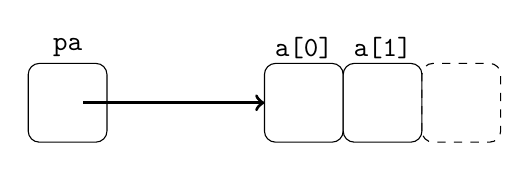
\begin{tikzpicture}
\draw[rounded corners] (0, 0) rectangle (1, 1) {};
\draw[rounded corners] (1, 0) rectangle (2, 1) {};
\draw[rounded corners,dashed] (2, 0) rectangle (3, 1) {};
\node at (0.5,1.2) {\texttt{a[0]}};
\node at (1.5,1.2) {\texttt{a[1]}};

\draw[rounded corners] (-3, 0) rectangle (-2, 1) {};
\draw[very thick,->] (-2.3,0.5) -- (0,0.5);
\node at (-2.5,1.2) {\texttt{pa}};
\end{tikzpicture}
\end{center}

\begin{minted}{c}
pa = &a[1];
pa = (a+1);
\end{minted}

\begin{center}
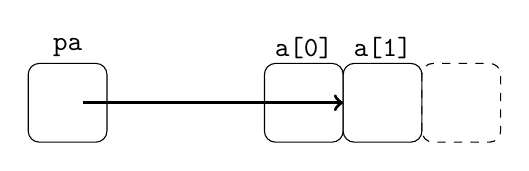
\begin{tikzpicture}
\draw[rounded corners] (0, 0) rectangle (1, 1) {};
\draw[rounded corners] (1, 0) rectangle (2, 1) {};
\draw[rounded corners,dashed] (2, 0) rectangle (3, 1) {};
\node at (0.5,1.2) {\texttt{a[0]}};
\node at (1.5,1.2) {\texttt{a[1]}};

\draw[rounded corners] (-3, 0) rectangle (-2, 1) {};
\draw[very thick,->] (-2.3,0.5) -- (1,0.5);
\node at (-2.5,1.2) {\texttt{pa}};
\end{tikzpicture}
\end{center}

\item The two pairs of statements above are equivalent using array or pointer notation: \verb!+1! translates to \verb!+4! bytes (1 \verb!int!)
\end{itemize}



\section{Recap --- Strange but true}
\begin{itemize}
\item In C if I write \verb!a[x]! this works by adding \verb!x! to \verb!a! to find the pointer
\item Hence \verb!a[x]! is the same as \verb!*(a+x)!
\item This seems fine if I write \verb!a[2]!
\item But what if I write \verb!2[a]!?
\item It compiles and works!
\end{itemize}



\begin{itemize}
\item We can also have multi-dimensional arrays in C e.g.
\begin{minted}{c}
int matrix[2][3] = {{1,2,3},{4,5,6}};
\end{minted}
\item Now \verb!matrix[0][1]==2!
\item Can have more than 2-dimensional arrays:
\begin{minted}{c}
int arr3d[3][2][4] = {
    {{1, 2, 3, 4}, {5, 6, 7, 8}},
    {{9, 10, 11, 12}, {13, 14, 15, 16}},
    {{17, 18, 19, 20}, {21, 22, 23, 24}}
};
\end{minted}
\item The elements of \verb!arr3d! will be allocated in memory in the order \verb!arr3d[0][0][0]!,  \verb!arr3d[0][0][1]!,  \verb!arr3d[0][0][2]!,  \verb!arr3d[0][0][3]!,  \verb!arr3d[0][1][0]!,  \verb!arr3d[0][1][1]! etc.
\end{itemize}



\begin{minted}{c}
int arr3d[3][2][4] = {
    {{1, 2, 3, 4}, {5, 6, 7, 8}},
    {{9, 10, 11, 12}, {13, 14, 15, 16}},
    {{17, 18, 19, 20}, {21, 22, 23, 24}}
};
\end{minted}
\begin{itemize}
\item Now \verb!&arr3d[i][j][k]! is the same as \verb!&arr3d[0][0][0]+(i*2*4)+j*4+k!
\item What is the type of \verb!arr3d[0][0][0]!?
\item What is the type of \verb!arr3d[0][0]!?
\item What is the type of \verb!arr3d[0]!?
\item What is the type of \verb!arr3d!?
\item What does \verb!int (*p)[2][4]=arr3d;! do?
\item For further fun with pointers and arrays, read \url{https://www.oreilly.com/library/view/understanding-and-using/9781449344535/ch04.html}
\end{itemize}

\end{document}
